\documentclass[14pt]{beamer}
\usepackage[T2A]{fontenc}
\usepackage[utf8]{inputenc}
\usepackage[english,russian]{babel}
\usepackage{amssymb,amsfonts,amsmath,mathtext}
\usepackage{cite,enumerate,float,indentfirst}

\graphicspath{{images/}}

\usetheme{Pittsburgh}
\usecolortheme{whale}

\setbeamercolor{footline}{fg=blue}
\setbeamertemplate{footline}{
  \leavevmode%
  \hbox{%
  \begin{beamercolorbox}[wd=.333333\paperwidth,ht=2.25ex,dp=1ex,center]{}%
    Софийски университет
  \end{beamercolorbox}%
  \begin{beamercolorbox}[wd=.333333\paperwidth,ht=2.25ex,dp=1ex,center]{}%
    София, 2016
  \end{beamercolorbox}%
  \begin{beamercolorbox}[wd=.333333\paperwidth,ht=2.25ex,dp=1ex,right]{}%
  Стр. \insertframenumber{} из \inserttotalframenumber \hspace*{2ex}
  \end{beamercolorbox}}%
  \vskip0pt%
}

\newcommand{\itemi}{\item[\checkmark]}

\title{\small{Математически епидемиологически модели}}
\author{\small{%
\emph{Христо Вригазов}~\\%
\emph{Илия Жечев}~\\%
\emph{Виктор Божилов}~}\\%
\vspace{30pt}%
Приложение на математиката\\
за моделиране на реалните процеси%
\vspace{20pt}%
}
\date{\small{София, 2016}}

\begin{document}

\maketitle

\begin{frame}
\frametitle{Теми}
\begin{itemize}
  \item \textbf{SAIC модел}
  \item \textbf{Разширение на SIR модела} 
\end{itemize}
\end{frame}

\begin{frame}
\frametitle{Система, описваща модела}
    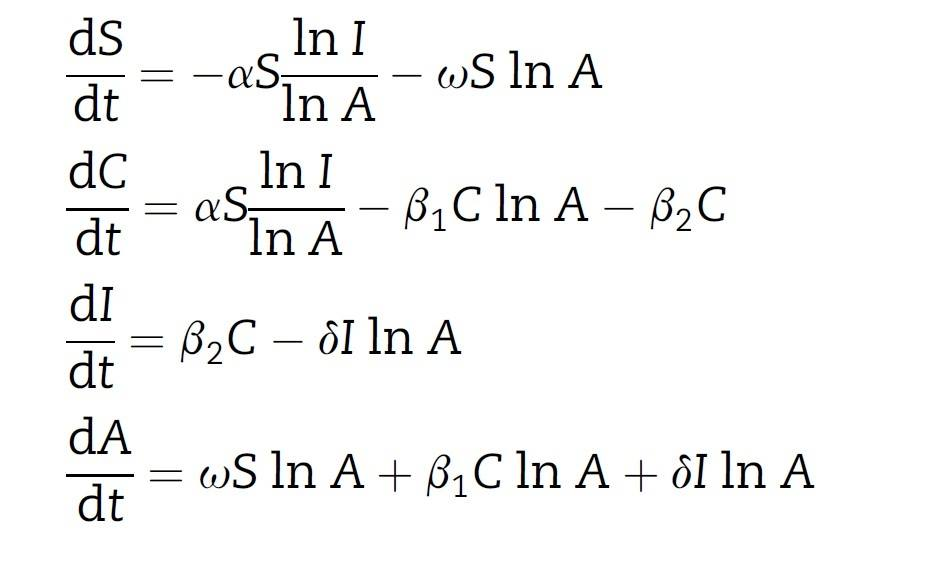
\includegraphics[width=0.8\linewidth] {pesa1}
\end{frame}

\begin{frame}
\frametitle{Система, описваща модела}
    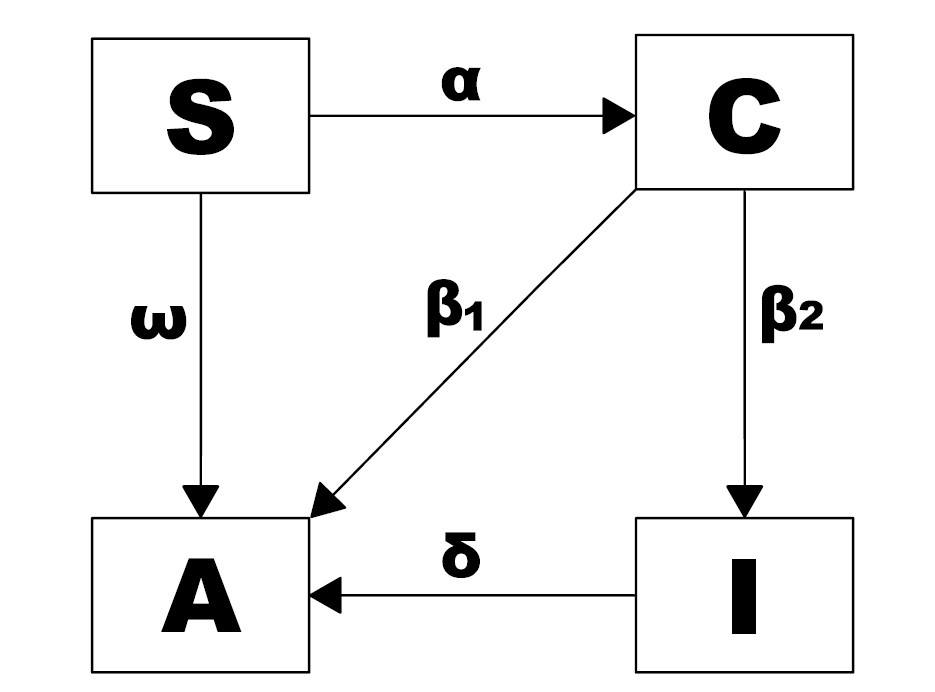
\includegraphics[width=0.8\linewidth] {pesa2}
\end{frame}

\begin{frame}
\frametitle{Графика на модела}
    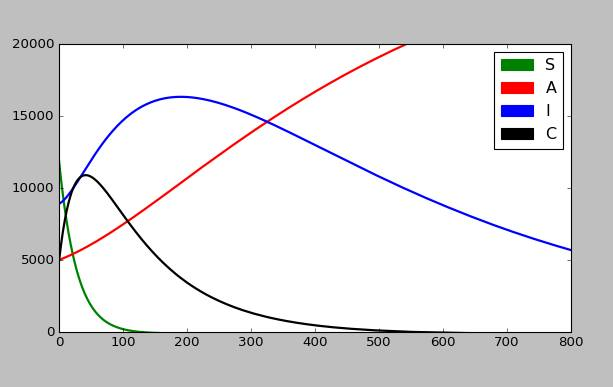
\includegraphics[width=0.8\linewidth] {pesa3}
\end{frame}

\begin{frame}
\frametitle{Разширен SIR модел}
Допускания
\begin{itemize}
    \item {Хората се движат на 2D терен, заразяват се в околност}
    \item {Човек може да роди с определена вероятност}
    \item {Човек може да умре с определена вероятност}
    \item {Човек остарява с определена скорост}
    \item {Болестта се характеризира с определена смъртоносност}
    \item {Болестта (не)? се предава от майка на дете}
    \item {Лекарство - имунизира човек с определена вероятност}
\end{itemize}
\end{frame}

\begin{frame}
\frametitle{Параметри}
    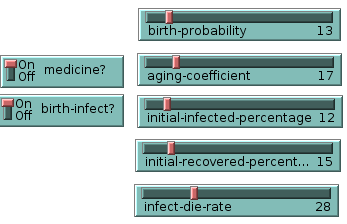
\includegraphics[width=0.8\linewidth] {parameters}
\end{frame}

\begin{frame}
\frametitle{Демо}
    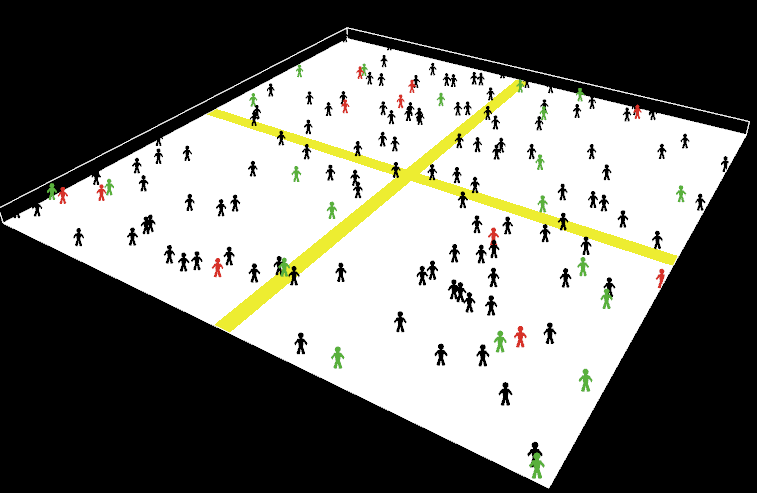
\includegraphics[width=0.8\linewidth] {demo}
\end{frame}

\begin{frame}
\frametitle{Бъдещи подобрения}
\begin{itemize}
    \item {Силата на лекарството да може да се контролира}
    \item {Преградите да спират хората}
    \item {Преминаванията от един град в друг да се параметризират}
\end{itemize}
\end{frame}

\begin{frame}
\begin{center}
Благодаря Ви за вниманието
\end{center}
\end{frame}

\end{document} 